\subsection*{Version your code}

The first step is to learn how to version your own code.
In this tutorial, we will run Git from the command line of the Unix shell.
Thus we expect readers are already comfortable with navigating a filesystem and running basic commands in such an environment.
You can find directions for installing Git for the operating system running on your computer by following one of the links provided in Table 1.
There are many graphical user interfaces (GUIs) available for running Git (Table 1), which we encourage you to explore, but learning to use Git on the command line is necessary for performing more advanced operations and using Git on a remote machine.

To follow along, first create a folder in your home directory named \verb|thesis|.
Next download the three files provided in Supporting Information and place them in the \verb|thesis| directory.
Imagine that as part of your thesis you are studying the transcription factor CTCF, and you want to identify high-confidence binding sites in kidney epithelial cells.
To do this, you will utilize publicly available ChIP-seq data produced by the ENCODE consortium \cite{22955616}.
ChIP-seq is a method for finding the sites in the genome where a transcription factor is bound, and these sites are referred to as peaks \cite{24244136}.
\verb|process.sh| downloads the ENCODE CTCF ChIP-seq data from multiple types of kidney samples and calls peaks,
\verb|clean.py| filters peaks with a fold change cutoff and merges peaks from the different kidney samples,
and \verb|analyze.R| creates diagnostic plots on the length of the peaks and their distribution across the genome.

If you have just installed Git, the first thing you need to do is provide some information about yourself, since it records who makes each change to the file(s).
Set your name and email by running the following lines, but replacing ``First Last'' and ``user@domain'' with your full name and email address, respectively.

\begin{verbatim}
$ git config --global user.name "First Last"
$ git config --global user.email "user@domain"
\end{verbatim}

To start versioning your code with Git, navigate to your newly created directory, \verb|~/thesis|.
Run the command \verb|git init| to initialize the current folder as a Git repository (Fig. \ref{fig:Fig1}, \ref{fig:Fig2}A).
A repository (or repo, for short) refers to the current version of the tracked files as well as all the previously saved versions (Box 1).
Only files that are located within this directory (and any subdirectories) have the potential to be version controlled,
i.e. Git ignores all files outside of the initialized directory.
For this reason, projects under version control tend to be stored within a single directory to correspond with a single Git repository.
For strategies on how to best organize your own projects, see Noble, 2009 \cite{19649301}.

\begin{figure}[h!]
\begin{center}
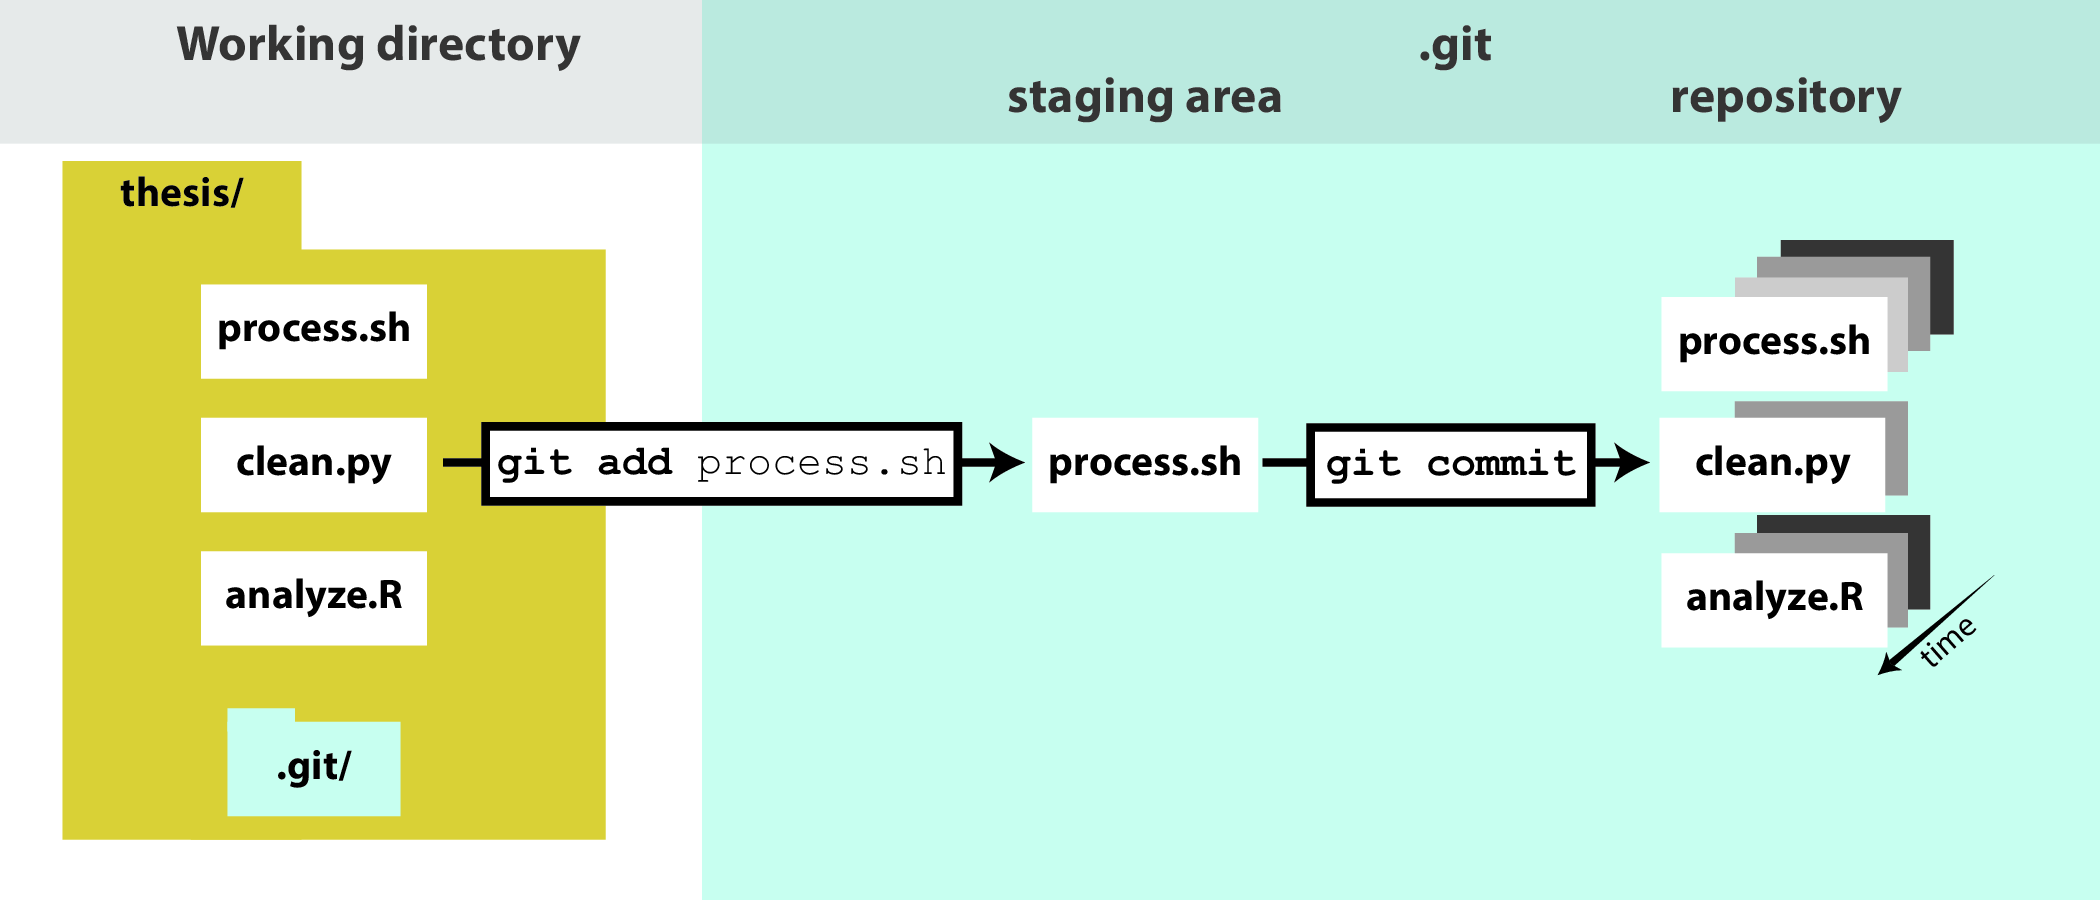
\includegraphics[width=1\columnwidth]{figures/Fig1/Fig1}
\caption{\textbf{\label{fig:Fig1}}%
}
\end{center}
\end{figure}

\begin{verbatim}
$ cd ~/thesis
$ ls
analyze.R clean.py process.sh
$ git init
Initialized empty Git repository in ~/thesis/.git/
\end{verbatim}

Now you are ready to start versioning your code (Fig. \ref{fig:Fig1}).
Conceptually, Git saves snapshots of the changes you make to your files whenever you instruct it to.
For instance, after you edit a script in your text editor, you save the updated script to your \verb|thesis| folder.
If you tell Git to save a shapshot of the updated document, then you will have a permanent record of the file in that exact version even if you make subsequent edits to the file.
In the Git framework, any changes you have made to a script, but have not yet recorded as a snapshot with Git, reside in the working directory only (Fig. \ref{fig:Fig1}).
To follow what Git is doing as you record the initial version of your files, use the informative command \verb|git status|.

\begin{verbatim}
$ git status
On branch master

Initial commit

Untracked files:
  (use "git add <file>..." to include in what will be committed)

        analyze.R
        clean.py
        process.sh

nothing added to commit but untracked files present (use "git add" to track)
\end{verbatim}

There are a few key things to notice from this output.
First, the three scripts are recognized as untracked files because you have not told Git to start tracking anything yet.
Second, the word ``commit'' is Git terminology for snapshot.
As a noun it means ``a version of the code'', e.g. ``the figure was generated using the commit from yesterday'' (Box 1).
This word can also be used as a verb, in which case it means ``to save'', e.g. ``to commit a change.''
Lastly, the output explains how you can track your files using \verb|git add|.
Start tracking the file \verb|process.sh|.

\begin{verbatim}
$ git add process.sh
\end{verbatim}

And check its new status.

\begin{verbatim}
$ git status
On branch master

Initial commit

Changes to be committed:
  (use "git rm --cached <file>..." to unstage)

        new file:   process.sh

Untracked files:
  (use "git add <file>..." to include in what will be committed)

        analyze.R
        clean.py
\end{verbatim}

Since this is the first time that you have told Git about the file \verb|process.sh|, two key things have happened.
First, this file is now being tracked, which means Git recognizes it as a file you wish to be version controlled (Box 1).
Second, the changes made to the file (in this case the entire file because it is the first commit) have been added to the staging area (Fig. \ref{fig:Fig1}).
Adding a file to the staging area will result in the changes to that file being included in the next commit, or snapshot of the code (Box 1).
As an analogy, adding files to the staging area is like putting things in a box to mail off, and committing is like putting the box in the mail.

Since this will be the first commit, or first version of the code, use \verb|git add| to begin tracking the other two files and add their changes to the staging area as well.
Then create the first commit using the command \verb|git commit|.

\begin{verbatim}
$ git add clean.py analyze.R
$ git commit -m "Add initial version of thesis code."
[master (root-commit) 660213b] Add initial version of thesis code.
 3 files changed, 154 insertions(+)
 create mode 100644 analyze.R
 create mode 100644 clean.py
 create mode 100644 process.sh
\end{verbatim}

Notice the flag \verb|-m| was used to pass a message for the commit.
This message describes the changes that have been made to the code and is required.
If you do not pass a message at the command line, the default text editor for your system will open so you can enter the message.
You have just performed the typical development cycle with Git:
make some changes, add updated files to the staging area, and commit the changes as a snapshot once you are satisfied with them (Fig. \ref{fig:Fig2}).

Since Git records all of the commits, you can always look through the complete history of a project.
To view the record of your commits, use the command \verb|git log|.
For each commit, it lists the unique identifier for that revision, author, date, and commit message.

\begin{verbatim}
$ git log
commit 660213b91af167d992885e45ab19f585f02d4661
Author: First Last <user@domain>
Date:   Fri Aug 21 14:52:05 2015 -0500

    Add initial version of thesis code.
\end{verbatim}

The commit identifier can be used to compare two different versions of a file, restore a file to a previous version from a past commit, and even retrieve tracked files if you accidentally delete them.

Now you are free to make changes to the files knowing that you can always revert them to the state of this commit by referencing its identifier.
As an example, edit \verb|clean.py| so that the fold change cutoff for filtering peaks is more stringent.
Here is the current bottom of the file.

\begin{verbatim}
$ tail clean.py
# Filter based on fold-change over control sample
fc_cutoff = 10
epithelial = epithelial.filter(filter_fold_change, fc = fc_cutoff).saveas()
proximal_tube = proximal_tube.filter(filter_fold_change, fc = fc_cutoff).saveas()
kidney = kidney.filter(filter_fold_change, fc = fc_cutoff).saveas()
# Identify only those sites that are peaks in all three tissue types
combined = pybedtools.BedTool().multi_intersect(
           i = [epithelial.fn, proximal_tube.fn, kidney.fn])
union = combined.filter(lambda x: int(x[3]) == 3).saveas()
union.cut(range(3)).saveas(data + "/sites-union.bed")
\end{verbatim}

Using a text editor, increase the fold change cutoff from 10 to 20.

\begin{verbatim}
$ tail clean.py
# Filter based on fold-change over control sample
fc_cutoff = 20
epithelial = epithelial.filter(filter_fold_change, fc = fc_cutoff).saveas()
proximal_tube = proximal_tube.filter(filter_fold_change, fc = fc_cutoff).saveas()
kidney = kidney.filter(filter_fold_change, fc = fc_cutoff).saveas()
# Identify only those sites that are peaks in all three tissue types
combined = pybedtools.BedTool().multi_intersect(
           i = [epithelial.fn, proximal_tube.fn, kidney.fn])
union = combined.filter(lambda x: int(x[3]) == 3).saveas()
union.cut(range(3)).saveas(data + "/sites-union.bed")
\end{verbatim}

Because Git is tracking \verb|clean.py|, it recognizes that the file has been changed since the last commit.

\begin{verbatim}
$ git status
# On branch master
# Changes not staged for commit:
#   (use "git add <file>..." to update what will be committed)
#   (use "git checkout -- <file>..." to discard changes in working directory)
#
#       modified:   clean.py
#
no changes added to commit (use "git add" and/or "git commit -a")
\end{verbatim}

The report from \verb|git status| indicates that the changes to \verb|clean.py| are not staged, i.e. they are in the working directory (Fig. 1).
To view the unstaged changes, run the command \verb|git diff|.

\begin{verbatim}
$ git diff
diff --git a/clean.py b/clean.py
index 7b8c058..76d84ce 100644
--- a/clean.py
+++ b/clean.py
@@ -28,7 +28,7 @@ def filter_fold_change(feature, fc = 1):
         return False

 # Filter based on fold-change over control sample
-fc_cutoff = 10
+fc_cutoff = 20
 epithelial = epithelial.filter(filter_fold_change, fc = fc_cutoff).saveas()
 proximal_tube = proximal_tube.filter(filter_fold_change, fc = fc_cutoff).saveas()
 kidney = kidney.filter(filter_fold_change, fc = fc_cutoff).saveas()
\end{verbatim}

Any lines of text that have been added to the script are indicated with a \verb|+| and any lines that have been removed with a \verb|-|.
Here, we altered the line of code which sets the value of \verb|fc_cutoff|.
\verb|git diff| displays this change as the previous line being removed and a new line being added with our update incorporated.
You can ignore the first five lines of output because they are directions for other software programs that can merge changes to files.
If you wanted to keep this edit, you could add \verb|clean.py| to the staging area using \verb|git add| and then commit the change using \verb|git commit|, as you did above.
Instead, this time undo the edit by following the directions from the output of \verb|git status| to ``discard changes in the working directory'' using the command \verb|git checkout|.

\begin{verbatim}
$ git checkout -- clean.py
$ git diff
\end{verbatim}

Now \verb|git diff| returns no output because \verb|git checkout| undid the unstaged edit you had made to \verb|clean.py|.
And this ability to undo past edits to a file is not limited to unstaged changes in the working directory.
If you had committed multiple changes to the file \verb|clean.py| and then decided you wanted the original version from the initial commit, you could replace the argument \verb|--| with the commit identifier of the first commit you made above (your commit identifier will be different; use \verb|git log| to find it).
The \verb|--| used above was simply a placeholder for the first argument because by default \verb|git checkout| restores the most recent version of the file from the staging area (if you haven't staged any changes to this file, as is the case here, the version of the file in the staging area is identical to the version in the last commit).
Instead of using the entire commit identifier, use only the first seven characters, which is simply a convention since this is usually long enough for it to be unique.

\begin{verbatim}
$ git checkout 660213b clean.py
\end{verbatim}

At this point, you have learned the commands needed to version your code with Git.
Thus you already have the benefits of being able to make edits to files without copying them first, to create a record of your changes with accompanying messages, and to revert to previous versions of the files if needed.
Now you will always be able to recreate past results that were generated with previous versions of the code (see the command \verb|git tag| for a method to facilitate finding specific past versions) and see the exact changes you have made over the course of a project.
